% \FloatBarrier

\section{评估}
\label{sec:evaluation}


\begin{figure*}[htbp]
  \centering
  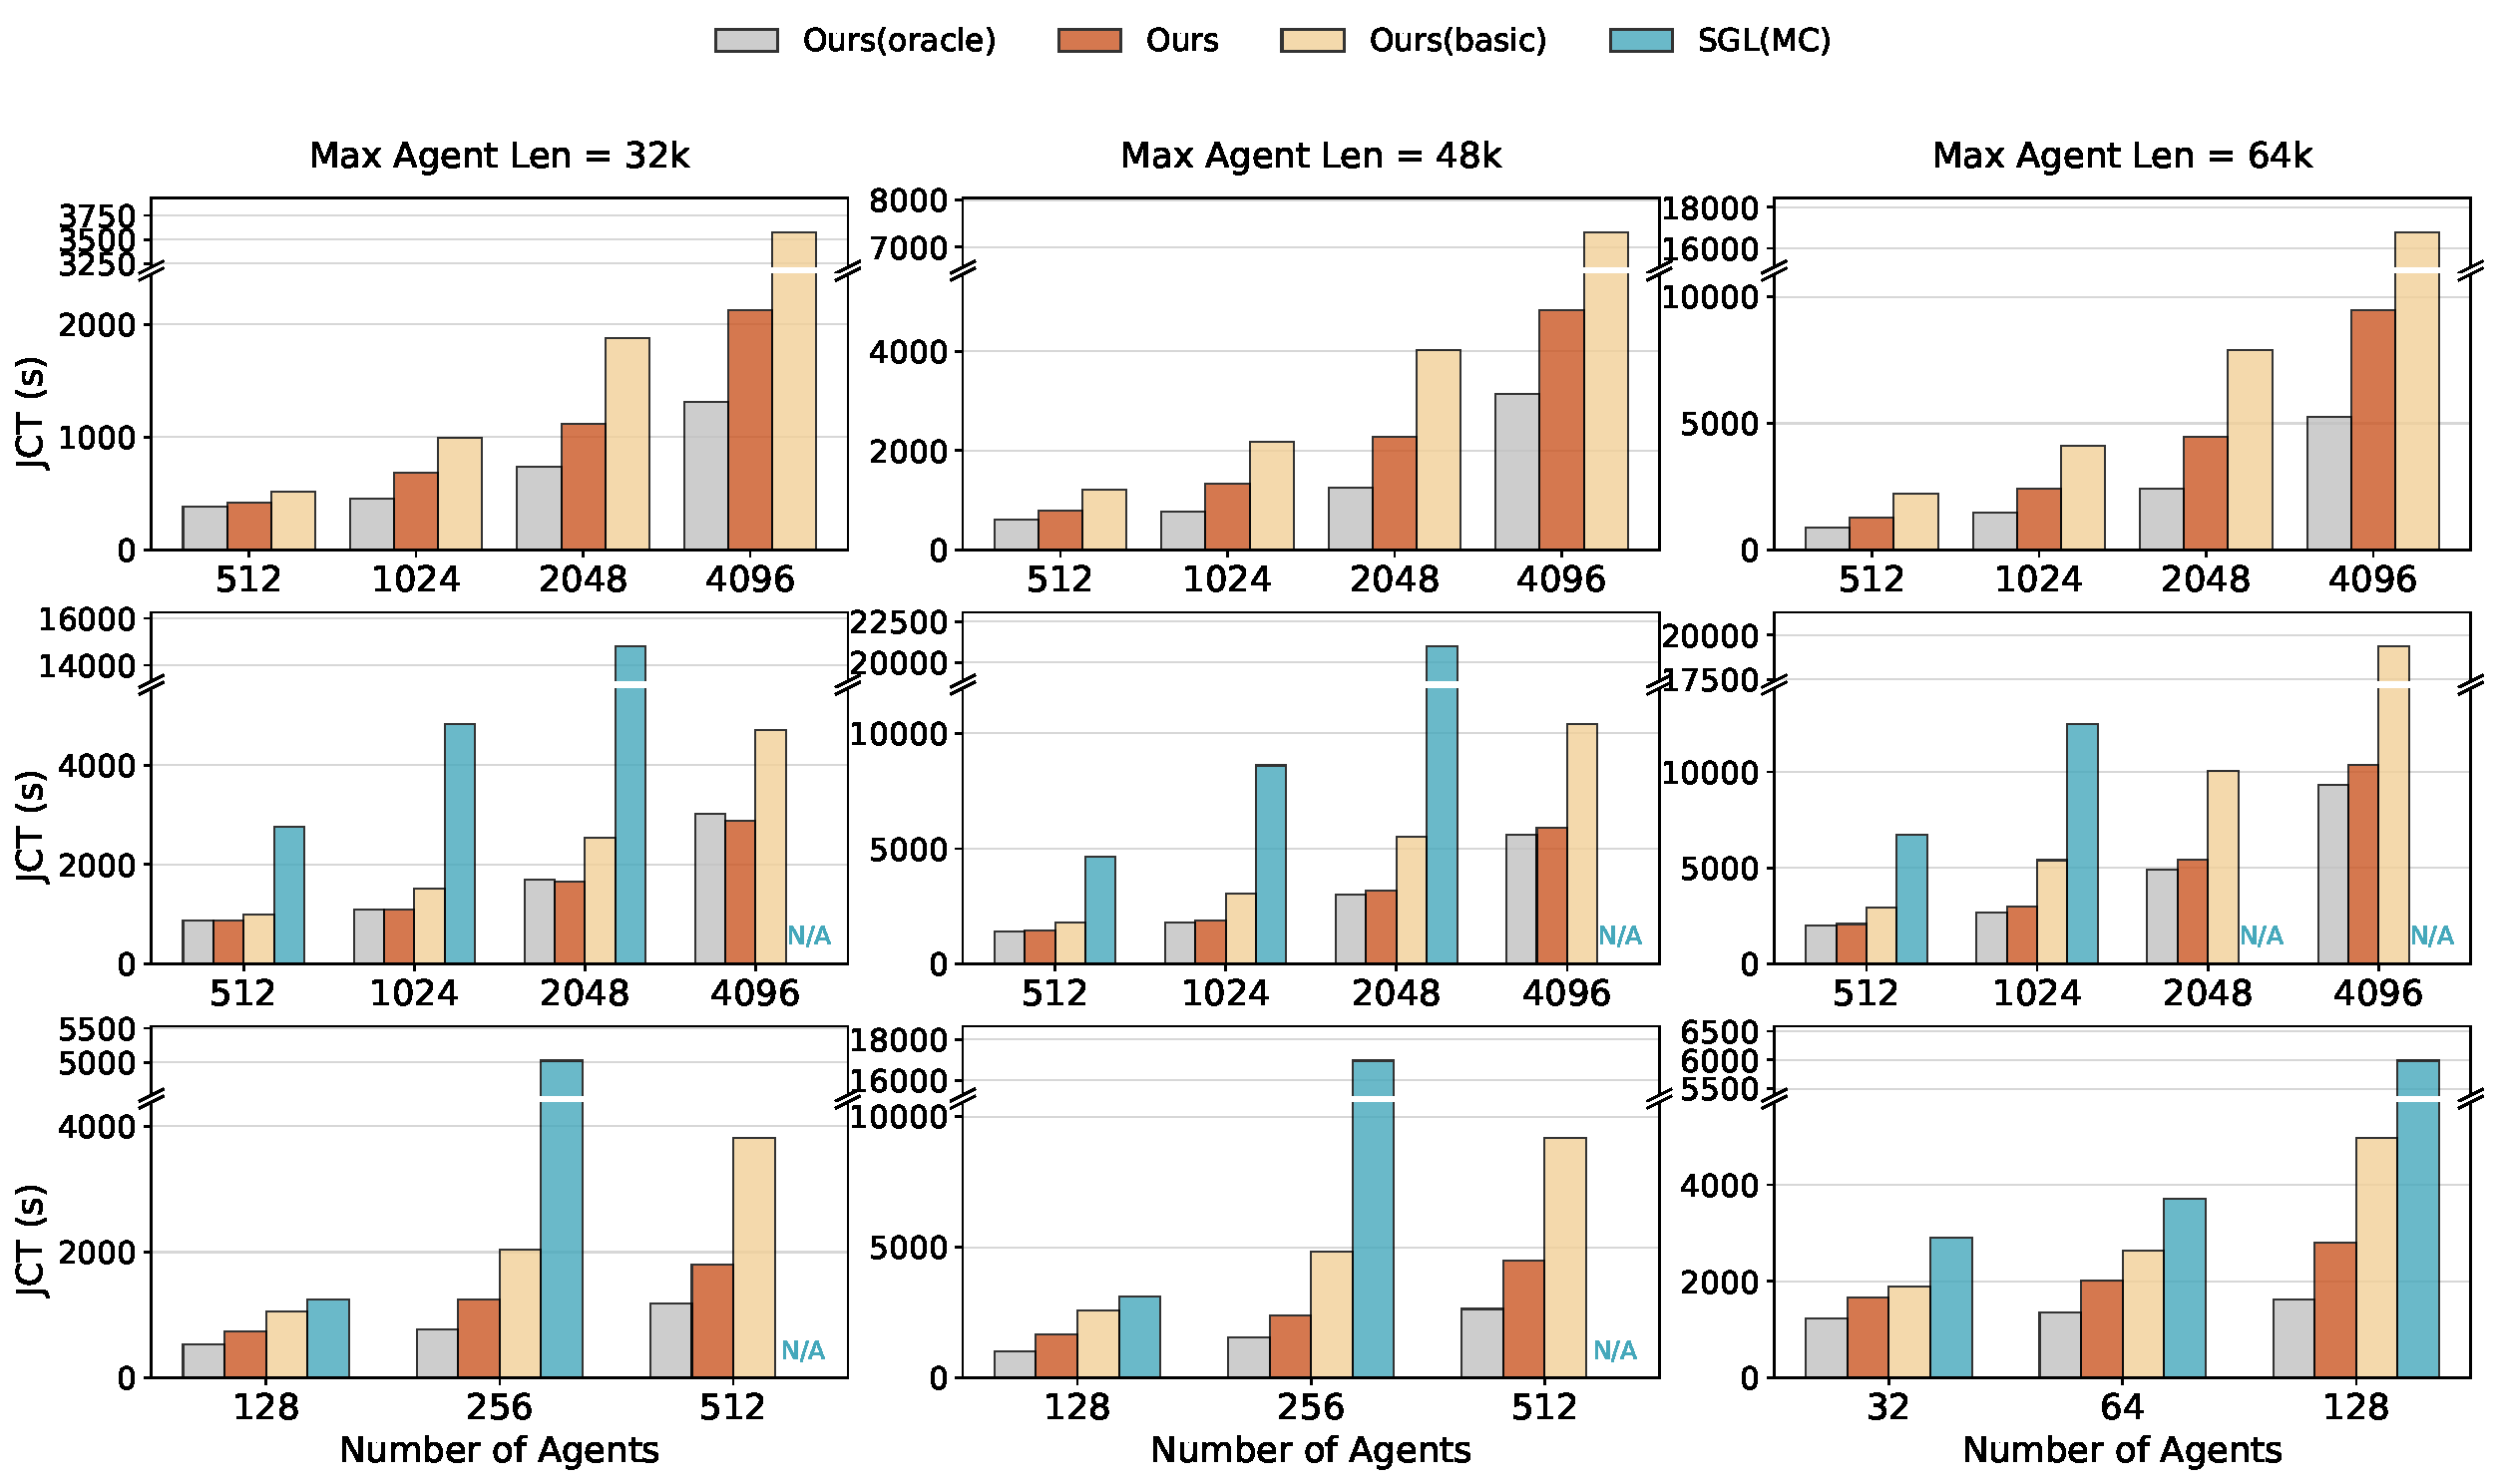
\includegraphics[width=0.98\linewidth]{figures/rollout_combined}
  \caption{\normalfont 不同智能体数量和最大智能体上下文长度下的离线推理性能。上：DS 27B。中：DS 660B。下：Qwen 32B。N/A 表示完成前遇到错误。}
  \label{fig:rollout}
\end{figure*}


\subsection{实现}
\label{subsec:impl}
我们基于内部推理框架实现 \sysname。
对于 CUDA kernel，我们的内部框架采用 FlashMLA~\cite{FlashMLA}、DeepGEMM~\cite{DeepGEMM} 和 DeepEP~\cite{DeepEP} 的组合，这与当前主流开源框架~\cite{NIPS24:SGLang, SOSP23:PagedAttention} 保持一致。
\sysname 的实现大约在该框架之上修改了 5K 行代码。
我们采用 3FS~\cite{3FS} 作为分布式存储，并使用类似 \verb|io_uring| 的接口实现 kernel bypass。

\subsection{实验设置}
\label{subsec:experimental-setup}

\paraf{测试平台。}
我们在一个使用 InfiniBand 互连的 GPU 服务器集群上进行实验。每台服务器配备 8 块 NVIDIA Hopper GPU 和双路处理器。此外，每个节点配置 8 张连接到 InfiniBand 网络的 400Gbps RDMA NIC，以及一张额外连接到 3FS 的存储 NIC。计算网络和存储网络在物理上隔离。我们的集群级 3FS 不包含内部 DRAM cache，并可打满存储 NIC 的 400Gbps 带宽。

\parabf{模型。}
我们评估三个模型：（1）DeepSeek V3.2~\cite{DeepSeekV32} 660B，一个带 DeepSeek Sparse Attention 的 MoE 模型，记为 \emph{DS 660B}；（2）DS 660B 的 27B 缩小版本，记为 \emph{DS 27B}；（3）Qwen2.5-32B~\cite{qwen2025qwen25technicalreport}，一个带 GQA 的 dense 模型，记为 \emph{Qwen 32B}。
DS 660B 和 Qwen 32B 对应 HuggingFace 上公开发布的 checkpoint。
DS 27B 是我们的内部实验模型，其架构与 DS 660B 类似。
详细规格见 \autoref{sec:27b-model-specs}。


\parabf{数据集。}
我们从生产智能体 RL 训练工作负载中收集了三个智能体 trace 数据集，最大上下文长度（MaxLen）不同。每个数据集包含 500 条轨迹。平均交互轮数（Turns）、每轮平均追加和生成 token 数（Append 和 Gen）、平均总 token 数（Total）以及平均上下文 token 数（Context）汇总于 \autoref{tab:agent-dataset-statistics}。

\begin{table}[t!]
\centering
\caption{\normalfont 智能体 trace 数据集统计。}
\begin{tabular}{cccccc}
\toprule
\textbf{MaxLen} & \textbf{Turns} & \textbf{Append} & \textbf{Gen} & \textbf{Total} & \textbf{Context} \\
\midrule
32K  &  60 & 608  & 148 & 28639 & 17183 \\
48K  & 106 & 474  & 172 & 42607 & 25120 \\
64K  & 157 & 429  & 176 & 55958 & 32721 \\
\bottomrule
\end{tabular}
\label{tab:agent-dataset-statistics}
\end{table}


\parabf{基线。}
我们将 \sysname（记为 Ours）与以下基线比较：

\begin{itemize}[leftmargin=*]
\item \textbf{SGL(MC)}：SGLang~\cite{NIPS24:SGLang}（commit 19089aa），启用 HiCache~\cite{Hicache}、Mooncake~\cite{FAST25:Mooncake} Store，并以 3FS 作为存储后端，同时使用 Mooncake Transfer Engine 支持 prefill-decode 解耦。
由于 SGLang 不支持 DS 27B 这个缩小版本，我们没有在 DS 27B 上运行 SGL(MC)。
\item \textbf{Basic}：未修改的内部推理框架（详见 \autoref{subsec:impl}）。
由于实现差异，直接比较 \sysname 和 SGL(MC) 并不公平。
因此，我们只报告从 Basic 到 Ours 的性能提升。
\item \textbf{Oracle}：基于 \sysname，但绕过所有磁盘读取、D2H 与 H2D 传输，以及 inter-PD KV-Cache 传输。
该配置代表假设 I/O 开销为零时的理论性能上界。
\end{itemize}

\parabf{P/D 比例与并行方式。} 
默认情况下，DS 660B 使用 2P4D，Qwen 32B 使用 1P2D，DS 27B 使用 1P1D（其中 1P1D 表示每一侧各用一个节点）。
对于 DS 模型，我们使用 EP 和 DP。
对于 Qwen 32B，\sysname 只使用 DP，而 SGL(MC) 使用 TP=8，因为 SGLang 中该模型不支持 DP attention。
详细配置见 \autoref{sec:experimental-configurations}。

\parabf{指标。} 对于离线推理场景，我们测量整个任务的 job completion time（JCT）。
对于在线服务场景，我们测量 TTFT、TTST（Time to the second token）和 TPOT。


\subsection{离线批量推理}
\label{subsec:offline-batch-infer}




本节评估离线批量推理中的吞吐量性能，该场景对应 RL 训练中的 rollout 阶段。
在该场景中，$n$ 个智能体同时开始 rollout，我们测量所有请求完成时的 JCT。

\parabf{改变智能体 Batch Size 与最大智能体长度（MAL）。}
\sysname 在更大 batch size 和更长 MAL 下受益更多。
\autoref{fig:rollout} 报告了不同 batch size 和 MAL 下的 JCT。
SGL(MC) 在我们的设置中遇到错误，无法完成部分大规模配置（标记为 N/A）。
在 DS 660B 上，\sysname 相比 Basic 最高达到 $1.87\times$，并展示出接近 Oracle 的性能，说明 KV-cache I/O 基本被消除。
在 DS 27B 上，\sysname 相比 Basic 最高提升 $1.78\times$，但由于 1P1D 下存储带宽有限，仍比 Oracle 慢 $1.09$--$1.85\times$（\autoref{fig:rollout_diff_pd}）。
Qwen 32B 展现出与 DS 27B 类似的趋势。





\begin{figure*}[htbp]
  \centering
  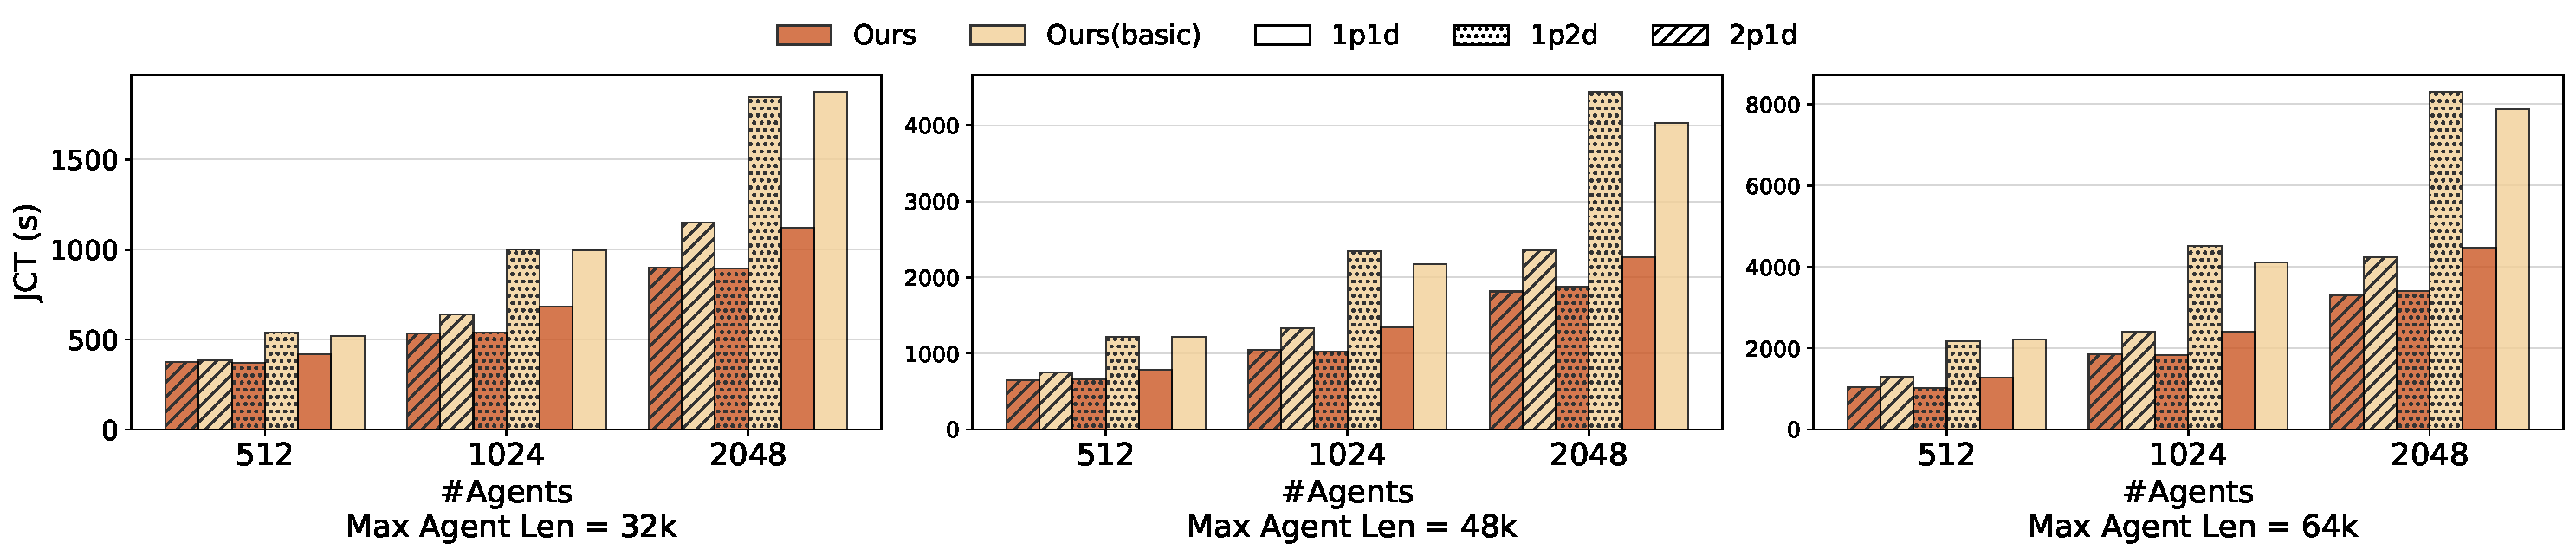
\includegraphics[width=\linewidth]{figures/27b_rollout_diffpd}\\
  \caption{\normalfont Prefill-decode 比例对离线推理性能的影响（DS 27B）。}
  \label{fig:rollout_diff_pd}
\end{figure*}



\begin{figure}[t]
  \centering
  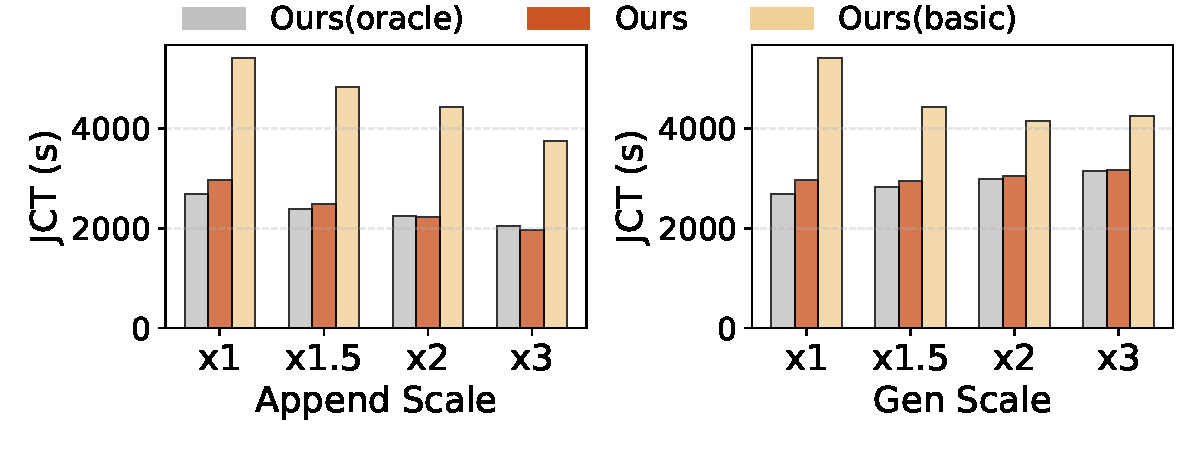
\includegraphics[width=\linewidth]{figures/660b_rollout_var_append_64k_traj512}
  \caption{\normalfont 左：不同追加长度（DS 660B，64K 上下文，1024 个智能体）。右：不同生成长度（DS 660B，64K，1024 个智能体）。}
  \label{fig:rollout_diff_append}
  \end{figure}




\begin{figure*}[htbp]
  \centering
  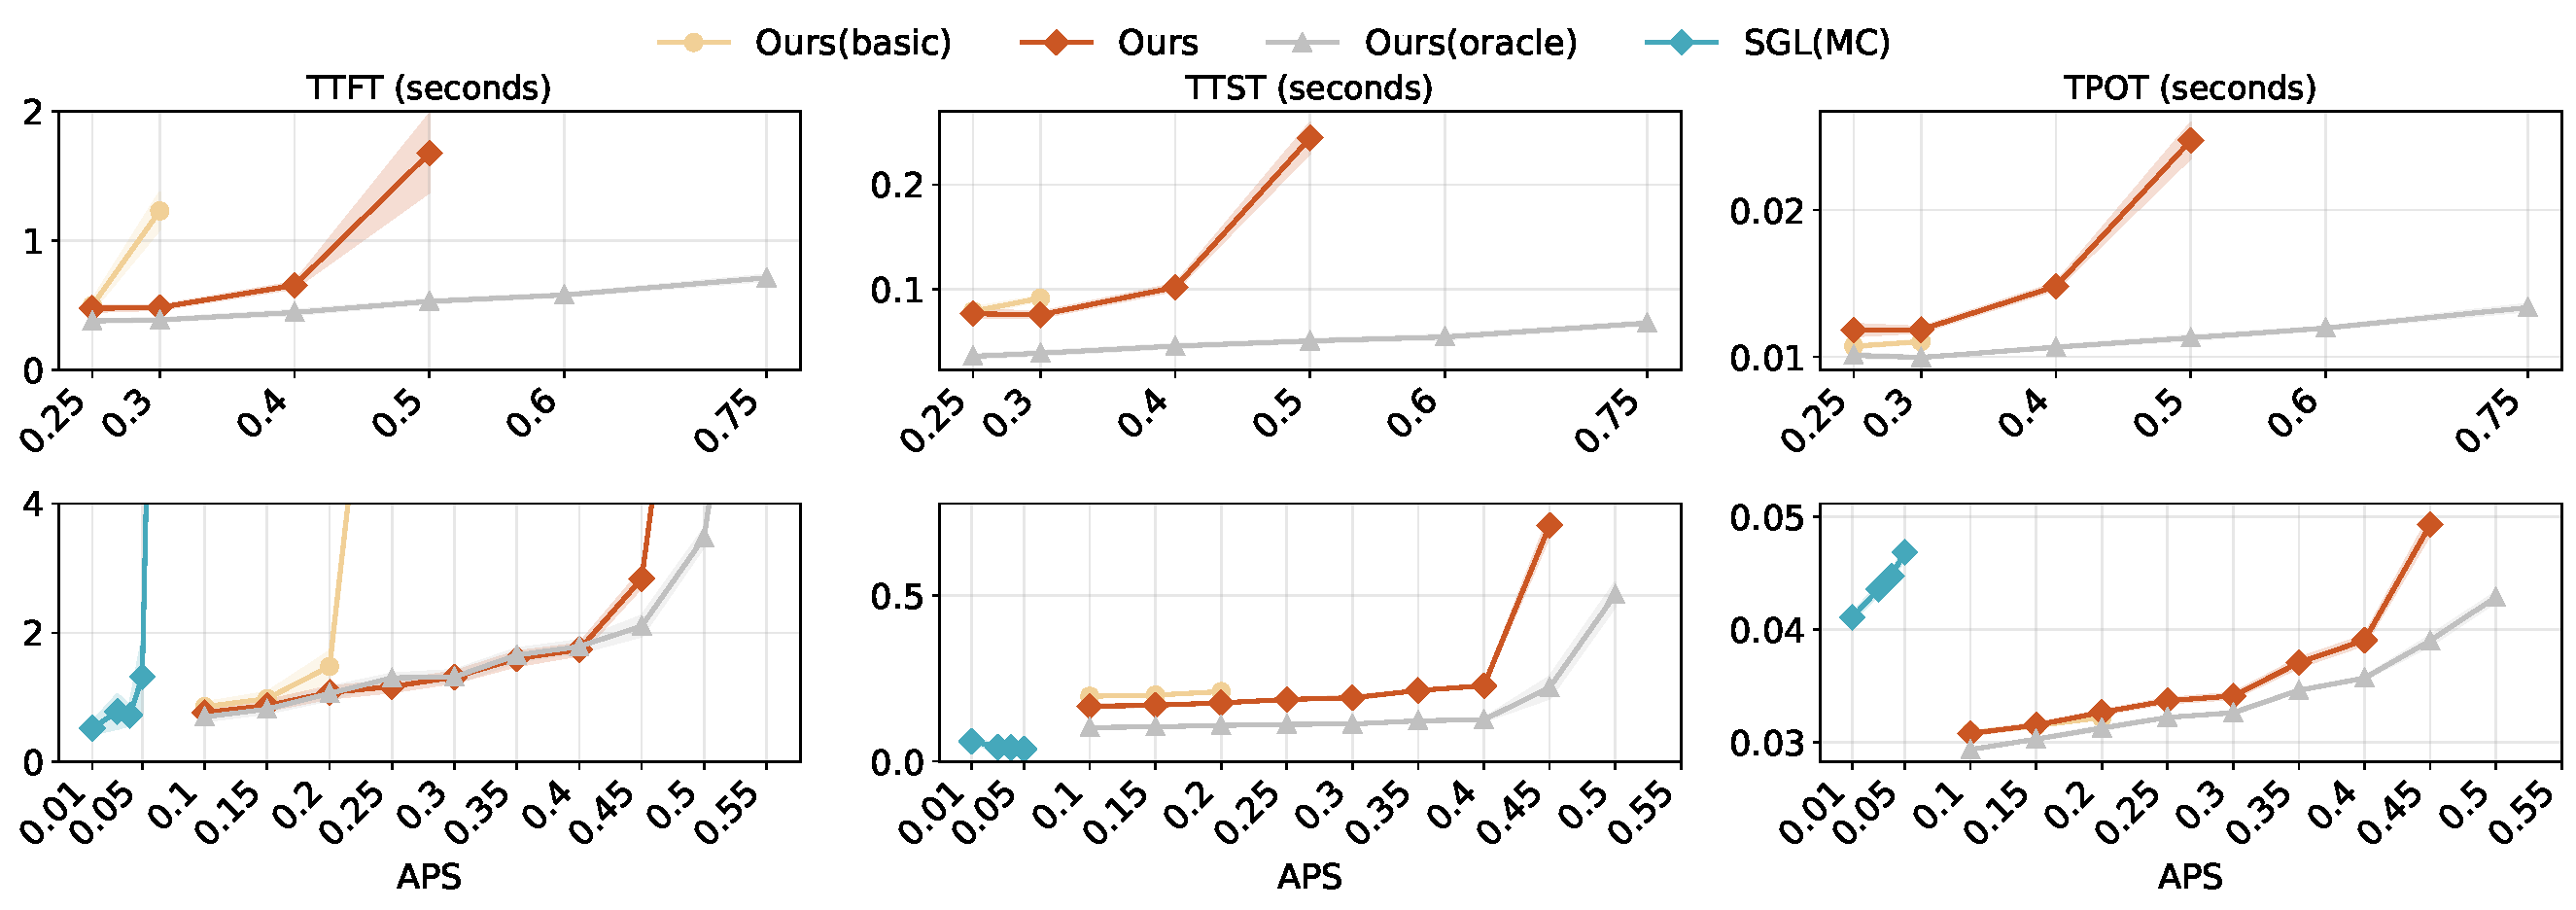
\includegraphics[width=0.88\linewidth]{figures/660b-27b-serving-aps-ttft-ttst-tpot}
  \vspace{-2mm}
  \caption{\normalfont TTFT、TTST 和 TPOT 随智能体到达率（APS）的变化。阴影表示实验结束前最后 150s 内的波动。上：DS 27B；下：DS 660B。}
  \label{fig:serving}
\end{figure*}

\parabf{改变追加长度与生成长度。}
当追加 token 和生成 token 较短时，\sysname 具有更大优势。
更长的追加长度意味着更高 GPU 计算压力；更长的生成长度则会由于更大的 prefill 间隔时间而降低 KV-Cache 加载压力。
为研究该因素影响，我们将每轮追加长度按常数因子缩放，然后在给定 MAL 处截断整条轨迹。
生成长度采用同样处理。
如 \autoref{fig:rollout_diff_append} 所示，随着追加长度增加，Basic 性能逐渐接近 \sysname 和 Oracle，而 \sysname 与 Oracle 性能变化很小，说明瓶颈持续位于 GPU 计算压力。
相比 Basic，\sysname 在不同追加长度缩放下获得 $1.82-1.99\times$ 加速。
生成长度缩放呈现类似趋势。




\parabf{改变 Prefill-Decode 比例。}
在所有比例下，\sysname 相比 Basic 都展现出显著性能收益。
我们在 DS 27B 上用 1P1D、2P1D 和 1P2D prefill-decode 比例进行 rollout 实验，以刻画 prefill 与 decode 阶段之间资源分配对系统整体性能的影响。
如 \autoref{fig:rollout_diff_pd} 所示，\sysname 在所有配置上平均加速 $1.64\times$（最高 $2.46\times$）。
Basic 1P1D 与 Basic 1P2D 表现相近；
\sysname 1P1D 与 Basic 2P1D 也相近，
\sysname 2P1D 与 \sysname 1P2D 同样相近。
这是因为每对系统拥有等价的可用存储带宽（Basic 只能使用 prefill 节点存储带宽，而 \sysname 可利用所有节点），这证明存储带宽是智能体场景中的主导瓶颈。



\subsection{在线服务}
\label{subsec:online-serving}
\parabf{方法。} 我们评估不同每秒智能体到达率（APS）下的系统延迟特征。
智能体按指定速率服从泊松过程到达；每个智能体到达后，从第 0 轮开始 replay 到最后一轮。
实验中，SLO 设置为 TTFT $\leq$ 4 秒且 TPOT $\leq$ 50ms。
在 TPOT 和 TTST 图中，超过 SLO 阈值的数据点被省略。
当出现以下任一情况时，实验终止：（1）TTFT 超过 4 秒；或（2）系统达到稳态，即 150 秒滑动窗口内 TTFT 变化相较 30 分钟前保持在 5\% 以下。



如 \autoref{fig:serving} 所示，\sysname 相比 Basic 可支持更高 APS 容量（DS 27B 为 1.67$\times$，DS 660B 为 2.25$\times$）。
\sysname 的 TTST 与 Basic 相当，而 TPOT 表明，相比 Basic，\sysname 不会引入额外 decode 开销。
SGL(MC) 表现出异常低的 TTST，这可能是实现问题导致的：前两个 token 几乎同时到达客户端。
对于 DS 27B，所有指标都呈现出与 DS 660B 类似的趋势。
然而，Basic 和 \sysname 的 TPOT 都显著高于 Oracle，说明在小模型场景下基础 P-D 传输开销相当可观。我们将其留作未来工作。


\begin{figure}[hbtp]
  \centering
  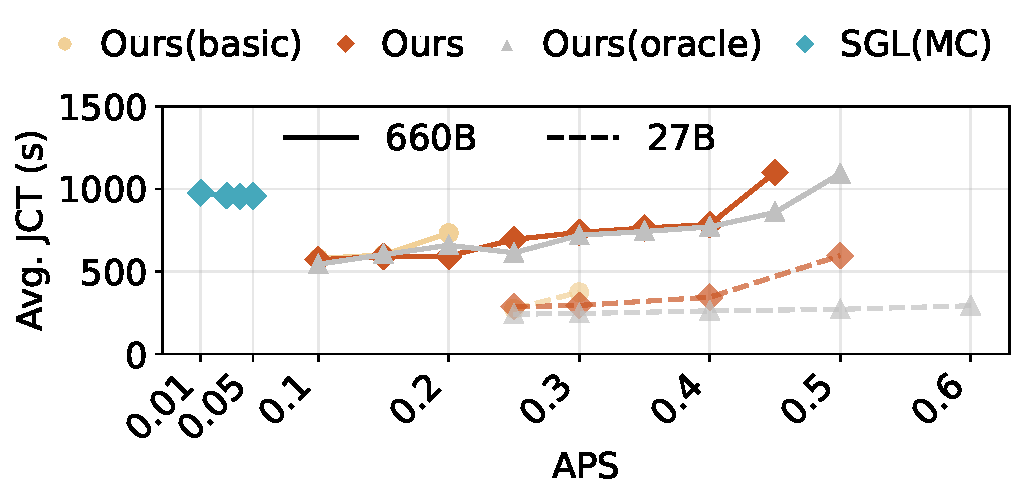
\includegraphics[width=0.9\linewidth]{figures/serving-aps-avg-jct}
  \vspace{-2mm}
  \caption{\normalfont 在线服务中，所有轨迹平均完成时间随到达率的变化。}
  \label{fig:serving-jct}
\end{figure}
两个模型的平均 JCT 如 \autoref{fig:serving-jct} 所示。
关于 working set 影响的详细分析见 \autoref{sec:discussion}。
如 \autoref{fig:ablation-and-ttft-breakdown}（左）所示，\sysname 在不同 APS 下保持稳定的 TTFT 组成，而 Basic 由于存储带宽不足，其排队时间急剧增长。



\subsection{消融研究}
\label{subsec:ablation}



\begin{figure}[t]
  \centering
  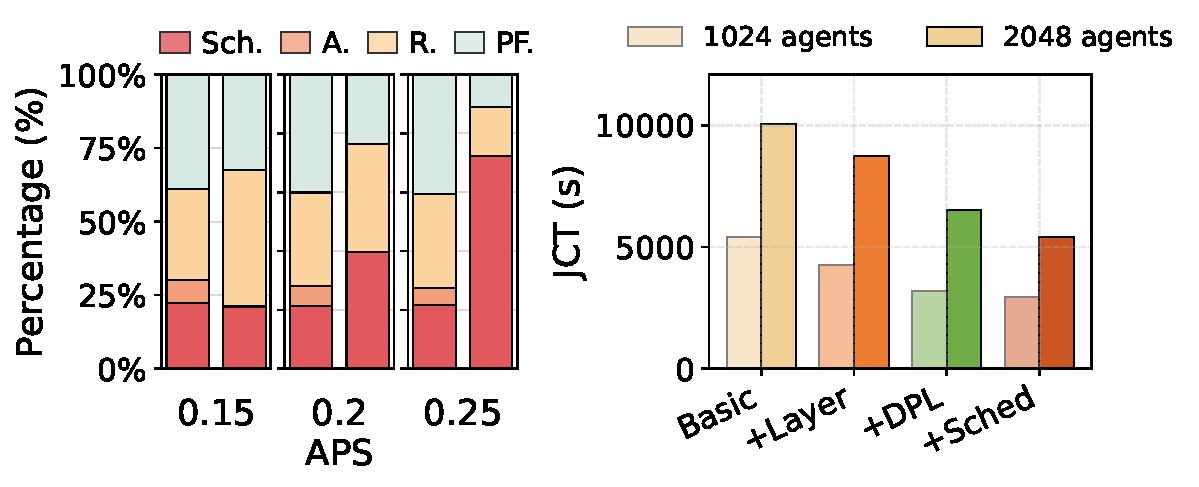
\includegraphics[width=\linewidth]{figures/660b_serving_breakdown}
  \caption{\normalfont 左（\autoref{subsec:online-serving}）：在线服务的 TTFT 细分（DS 660B），横跨不同 APS；Sch. 表示 scheduling，A. 表示 allocating，R. 表示 reading KV-cache，PF. 表示 prefill。每对柱子中，第一个为 \sysname，第二个为 Basic。右（\autoref{subsec:ablation}）：离线推理消融结果（DS 660B，64K 上下文长度）。Layer、DPL、Sched 分别表示 layerwise prefill、Dual-Path Loading 和 scheduling。}
  \label{fig:ablation-and-ttft-breakdown}
\end{figure}


我们进行消融研究，以量化 \sysname 中每个技术组件的贡献。
实验在离线推理设置下进行，MAL 为 64K，智能体 batch size 为 1024 和 2048。
Basic 与 Ours 之间的差异被分为三项技术：layerwise prefill、dual-path loading 和 scheduling algorithm。
我们逐步加入这些技术，以展示各自贡献。
如 \autoref{fig:ablation-and-ttft-breakdown} 所示，相比 Basic，加入 layerwise prefill 平均降低 JCT $17.21\%$，缓解 PE HBM 瓶颈并隐藏传输开销。
在 layerwise prefill 之上加入 Dual-path loading 带来主要性能收益，相比 Basic 平均降低 JCT $38.19\%$，因为它允许请求从 PE 或 DE 任一侧读取 KV-Cache，充分利用分布式存储带宽。
最后，在 dual-path loading 之上采用我们的调度算法来决定 KV-Cache 加载路径，可获得最佳性能，相比 Basic 降低 JCT $45.62\%$，证明跨存储 NIC 的负载均衡调度是有效的。



\begin{figure}[t]
  \centering
  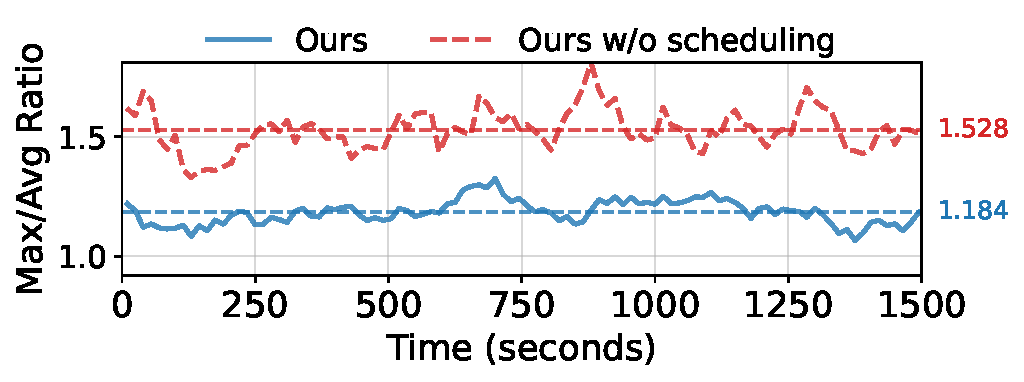
\includegraphics[width=0.9\linewidth]{figures/read_lb_48k_1024traj}
  \vspace{-3mm}
  \caption{\normalfont 存储 NIC 流量负载均衡。}
  %  with 64k MAL, 1024 agents batch size.
  \label{fig:read-lb}
\end{figure}



\begin{figure}[t]
  \centering
  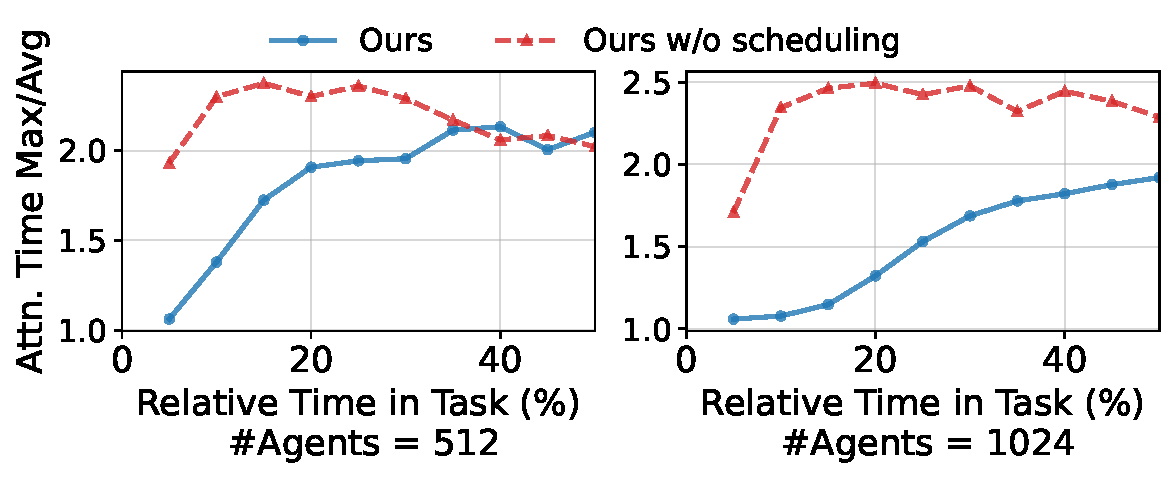
\includegraphics[width=\linewidth]{figures/attn_lb_48k}
  \caption{\normalfont Attention 执行时间的负载均衡。}
  \label{fig:attn-lb}
\end{figure}


\parabf{负载均衡。}
\sysname 的调度算法改善了存储 NIC 和 attention 层执行时间两方面的负载均衡。
对于存储 NIC，相比 round robin 调度，我们的调度算法将负载均衡指标从 1.53 改善到 1.18（\autoref{fig:read-lb}）。
对于 attention 层，在任务最初 5\% 期间，\sysname 将 Max/Avg 比率维持在低至 1.06，从而减少 GPU idle bubble（\autoref{fig:attn-lb}）。
存储 NIC 指标是在一个小时间窗口内，三台机器上所有存储 NIC 的最大流量与平均流量之比，其中 1.0 表示完美均衡。
Attention 层指标针对每个 forward，在 expert parallel group 内所有 GPU 之间计算。
随着任务推进，由于系统负载不足，两个比率都会失去意义。
因此，我们没有展示工作负载的尾部阶段。




\begin{table}[t]
  \centering
  \caption{\normalfont 大规模实验结果。}
  \label{tab:largescale}
  \setlength{\tabcolsep}{3pt}
  \small
  \begin{tabular}{cccccc}
  \toprule
  & \textbf{Setting} & \textbf{JCT} & \textbf{TTFT} & \textbf{TTST} & \textbf{TPOT} \\
  \midrule
  \multirow{2}{*}{\rotatebox{90}{\scriptsize Offline}} 
  & 2P4D, 2K agents & 3,167s & -- & -- & -- \\
  & 48P96D, 48K agents & 3,201s & -- & -- & -- \\
  \midrule
  \multirow{2}{*}{\rotatebox{90}{\scriptsize Online}} 
  & 2P4D, 0.4 APS & -- & 1.739s & 0.228s & 0.039s \\
  & 44P88D, 8.8 APS & -- & 1.847s & 0.194s & 0.036s \\
  \bottomrule
  \end{tabular}
  \end{table}

\begin{figure}[t]
  \centering
  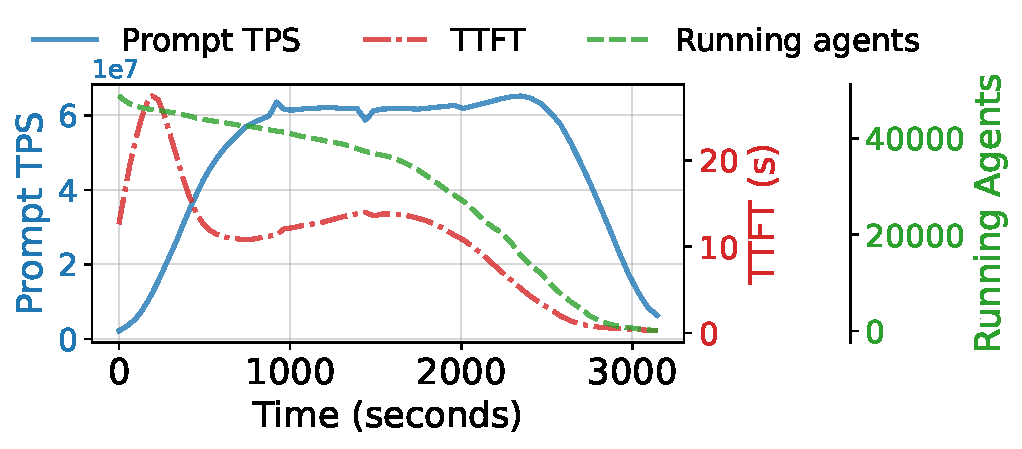
\includegraphics[width=\linewidth]{figures/largescale_rollout.pdf}
  \caption{\normalfont 48P96D 离线推理指标。1e7 是 Prompt TPS 的缩放因子。}
  \label{fig:largescale-rollout}
\end{figure}

\subsection{大规模可扩展性}



我们使用最多 1,152 块 GPU 进行离线和在线实验，以展示大规模可扩展性（\autoref{tab:largescale}）。
对于离线推理，从 2P4D（2K 个智能体）扩展到 48P96D（48K 个智能体）时，在相近 JCT 下获得近线性加速（3,167s vs.\ 3,201s）。
对于在线服务，44P88D 配置在保持相近延迟的同时实现 22$\times$ 吞吐量（8.8 vs.\ 0.4 APS）。
所有实验中，scheduler CPU 使用量始终低于 10 个 core，说明它不是瓶颈。离线推理过程中的若干详细指标见 \autoref{fig:largescale-rollout}。

由于缺少充分调优的并行设置和 P/D 比例（这需要大量实验预算），大规模实验并未相比等价成本下的多个小规模单元展示额外 JCT 或服务容量收益。
然而，大规模设置仍然重要，原因如下。第一，它减少碎片化，并为调优并行方式和 P/D 比例提供更大灵活性。第二，在不可预测的突发在线请求下，大规模部署提供更多调度机会来缓解排队延迟。这些观察指向若干未来工作方向（\autoref{subsec:futurework}）。

